\documentclass[12pt,a4paper]{report}
\usepackage[utf8]{inputenc}
\usepackage[spanish]{babel}
\usepackage{amsmath}
\usepackage{amsfonts}
\usepackage{amssymb}
\usepackage{makeidx}
\usepackage{graphicx}
\usepackage[left=1cm,top=1cm,right=1cm,bottom=1cm]{geometry} 
\title{Desarrollo}
\usepackage{float}
\begin{document}
	\begin{center}
		\begin{Large}
			Desarrollo.\\
			\vspace{2.5cm}
		\end{Large}
	\end{center}
\begin{flushleft}
	Lo primero que hicimos fue obtener los valores de cada una de las resitencias y compararlo con el  valor obtenido en la medici\'on, para ello nos apoyamos en una tabla del codigo de colores como la que se muestra a continuaci\'on:\\
	\vspace{0.5cm}
\begin{figure}[H]
	\centering
	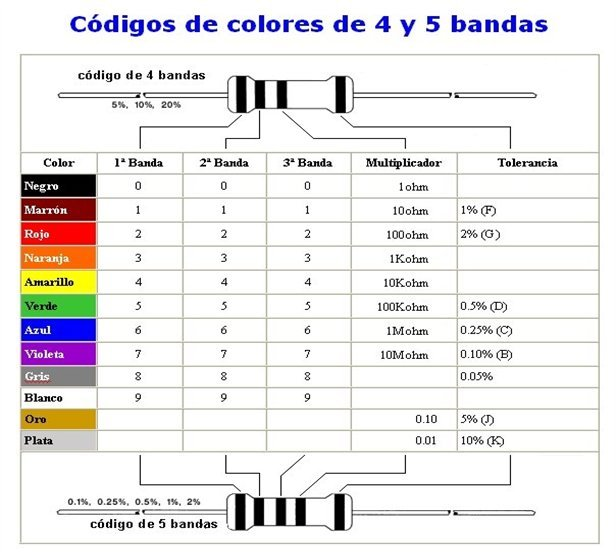
\includegraphics[width=0.4\linewidth]{bandas}
	\label{fig:bandas}
	\vspace{0.5cm}
\end{figure}
	
	\begin{large}
		Resistencia 1.
	\end{large}

	La primer muestra de resistencia que medimos fue de 




	
\end{flushleft}
	
\end{document}